% ******************************************************** %
%              TEMPLATE DE INFORME ORGA2 v0.1              %
% ******************************************************** %
% ******************************************************** %
%                                                          %
% ALGUNOS PAQUETES REQUERIDOS (EN UBUNTU):                 %
% ========================================
%                                                          %
% texlive-latex-base                                       %
% texlive-latex-recommended                                %
% texlive-fonts-recommended                                %
% texlive-latex-extra?                                     %
% texlive-lang-spanish (en ubuntu 13.10)                   %
% ******************************************************** %


\documentclass[hidelinks,a4paper,10pt, nofootinbib]{article}
\usepackage[spanish]{babel}
\usepackage[utf8]{inputenc}
\usepackage[T1]{fontenc}
\usepackage{hyperref} % links en índice
\usepackage{tabularx} % tablas copadas
\usepackage{charter}   % tipografia
\usepackage{graphicx}
\usepackage{amsmath, amsthm, amssymb}
\usepackage{listings}
%\usepackage{makeidx}
\usepackage{paralist} %itemize inline
\usepackage[table]{xcolor}

%\usepackage{float}
%\usepackage{amsfonts}
%\usepackage{sectsty}
%\usepackage{charter}
%\usepackage{wrapfig}

%\lstset{language=C}

% \setcounter{secnumdepth}{2}
\usepackage{underscore}
\usepackage{caratula}
\usepackage{url}


% ********************************************************* %
% ~~~~~~~~              Code snippets             ~~~~~~~~~ %
% ********************************************************* %

\usepackage{color} % para snipets de codigo coloreados
\usepackage{fancybox}  % para el sbox de los snipets de codigo

\definecolor{litegrey}{gray}{0.94}

\newenvironment{codesnippet}{%
	\begin{Sbox}\begin{minipage}{\textwidth}\sffamily\small}%
	{\end{minipage}\end{Sbox}%
		\begin{center}%
		\vspace{-0.4cm}\colorbox{litegrey}{\TheSbox}\end{center}\vspace{0.3cm}}



% ********************************************************* %
% ~~~~~~~~         Formato de las páginas         ~~~~~~~~~ %
% ********************************************************* %

\usepackage{fancyhdr}
\pagestyle{fancy}

%\renewcommand{\chaptermark}[1]{\markboth{#1}{}}
\renewcommand{\sectionmark}[1]{\markright{\thesection\ - #1}}

\fancyhf{}

\fancyhead[LO]{Sección \rightmark} % \thesection\ 
\fancyfoot[LO]{\small{Joel Esteban Cámera, Alejandro Lavía, Martin Jonas}}
\fancyfoot[RO]{\thepage}
\renewcommand{\headrulewidth}{0.5pt}
\renewcommand{\footrulewidth}{0.5pt}
\setlength{\hoffset}{-0.8in}
\setlength{\textwidth}{16cm}
%\setlength{\hoffset}{-1.1cm}
%\setlength{\textwidth}{16cm}
\setlength{\headsep}{0.5cm}
\setlength{\textheight}{25cm}
\setlength{\voffset}{-0.7in}
\setlength{\headwidth}{\textwidth}
\setlength{\headheight}{13.1pt}

\renewcommand{\baselinestretch}{1.1}  % line spacing

% ******************************************************** %


\begin{document}


\thispagestyle{empty}
\materia{Organización del Computador II}
\submateria{Primer Cuatrimestre de 2016}
\titulo{Trabajo Práctico II}
\subtitulo{Grupo: Más peligroso que mono con navaja}
\integrante{Joel Esteban Cámera}{257/14}{joel.e.camera@gmail.com}
\integrante{Alejandro Lavía}{43/11}{lavia.alejandro@gmail.com}
\integrante{Martin Jonas}{180/05}{martinjonas@gmail.com}

\maketitle
\newpage

%indice
\tableofcontents

\newpage

%\normalsize
\newpage

\section{Introducción}
El objetivo de este Trabajo Práctico es buscar una primera aproximación al modelo de procesamiento SIMD. Para esto este trabajo se compone de dos partes, la primera es de aplicar los conceptos aprendidos en clase sobre programación vectorizada y luego realizar un análisis experimental de los rendimientos obtenidos.

El campo de aplicación tomado es el procesamiento de imágenes. Para esto se nos encomendó la tarea de desarrollar en C y lenguaje de ensamblador tres filtros de imágenes, luego plantear hipótesis, experimentar y sacar conclusiones respecto de cada implementación.

El análisis de las implementaciones se lleva a cabo con un carácter científico y con las metodologías correspondientes.

Los filtros en cuestión fueron \textit{Cropflip}, \textit{Sepia} y \textit{Low-Dyn Range}.
El primero, es la unión de dos filtros: crop y vertical-flip. En donde dado una imagen, la cantidad de filas y columnas a cortar y la coordenada donde comenzar, genera una imagen de salida con la parte recortada de la imagen de entrada y volteada verticalmente.
El segundo, dado una imagen, genera una imagen de salida con la misma primer imagen pero con un cambio de color que se hace en cada uno de los pixels de la imagen de entrada. El tercero, dada una imagen y un coeficiente entero $\alpha$, aplica a un efecto a la imagen modificándola según su iluminación.

Para \textit{Cropflip}, se realizó el estudio de rendimiento entre la implementación en C y tres implementaciones en ASM de las cuales una de ellas es utilizando SIMD.
En el caso de \textit{Sepia}, también se realizó un estudio de rendimiento entre una implementación en C y dos implementaciones en ASM que utilizan SIMD.
En lo que respecta a \textit{Low-Dyn Range}, también se realizo la prueba de performance entre las dos implementaciones de C y otras tres implementaciones de ASM utilizando SIMD.

\newpage


\section{Desarrollo}
\subsection{Filtro Cropflip}

\textit{Cropflip} es un filtro muy sencillo en cuanto a su implementación, y el mas rápido en tiempo de ejecución debido a que no es necesario realizar ninguna modificación ni acceso diferenciado a las componentes del pixel.
Prácticamente se lo puede considerar como un caso de referencia para comparar rendimientos, debido a que lo que se realiza es una copia de memoria, sin necesidad de interpretar su contenido.

Para este filtro implementamos una versión en C y 3 versiones en ASM muy similares, pero con sutiles diferencias, pero con las cuales obtuvimos resultados muy diferentes.

\subsubsection{Cropflip - Versión 1 - C}
La implementación de la versión en C funciona con dos loops anidados, recorriendo desde offsetY una cantidad de tamY de filas, y desde el offsetX una cantidad tamX de columnas.
Luego para cada posición se copia al destino la estructura \textbf{bgra_t} completa.

\begin{lstlisting}[frame=single]
PTODO y <- RANGO[maxint..0] do { 

	PTODO x <- RANGO[0..tamX] do {
		DEST[ tamY - y - 1][x] <- SRC[ y + offsetY ][ x + offsetX ]
	}
}
\end{lstlisting}
\subsubsection{Cropflip - Versión 1/2/3 - ASM}

Las implementaciones de ASM trabajan sobre la imagen como un vector en vez de una matriz.
Para esto se manejan dos punteros. El de destino apuntando al principio de la ultima fila. 
Y en el de origen se saltean de la posición de memoria de inicio el offsetY * anchoFila * bytesPorPixel.

El ciclo de repite tamY veces y realiza lo siguiente:
\begin{enumerate}

\item Avanza el puntero de origen offsetX * bytesPorPixel.
\item Se copian del origen al destino la cantidad tamX de pixels.
\item Se saltean los pixels no copiados de la fila. 
	{\\ ((anchoDeFila - tamX - offsetX) * bytesPorPixel)}

\end{enumerate}

Las 3 versiones de ASM difieren en el punto 2 que es la forma de copiar los pixels. 
La versión 1 utiliza rep movsq (que repite la copia de quadwords)
La versión 2 realiza un ciclo copiando manualmente de [SRC] a un registro y luego a [DST]
La versión 3 realiza lo mismo que la 2 pero utilizando un registro XMM y por ende copiando de a 16 bytes.

\subsection{Filtro Sepia}
\textit{Sepia} es un filtro que requiere realizar una operación para cada pixel de forma independiente cambiando la información del color de estos, y después devolver el pixel al lugar que le pertenecía, generando en la imagen un color particular.
Para este filtro implementamos una versión en C y dos en ASM utilizando SIMD. Ambas implementaciones en ASM son símiles salvo en la forma de realizar las operaciones en cada pixel.
\subsubsection{Sepia - Versión 1 - C}

La implementación de la versión en C en donde simplemente recorre la estructura con dos ciclos anidados tomando cada uno de los pixels, generando el valor de \textbf{suma}, sumando cada una de las coordenadas de la tupla (sin contar los $\alpha$ que deben permanecer intactos en la operación), para luego agregar \textbf{suma} a cada una de las coordenadas multiplicándolo por el valor correspondiente a cada una ($0,5$ para el \textit{R}, $0,3$ para el \textit{G} y $0,2$ para el \textit{B}).

\begin{table}[h]
	\centering
	\begin{tabular}{| c | c | c | c |}
		\hline
		B & G & R & A  \\ \hline
		b0 & g0 & r0 & a0  \\ \hline
		\multicolumn{4}{|c|}{suma $=$ b0 + g0 + r0} \\ \hline
	\end{tabular}
\end{table}

Para la multiplicación, lo que se hizo fue tener dos variables temporales una en punto flotante (\textit{parte}) y otra en entero sin signo (\textit{tmp}). Dado que suma es entero sin signo, ya que cada elemento de la tupla lo es, la multiplicamos por el valor $0\text{.}1$f y alojamos el resultado en \textit{parte} ya que es en punto flotante el mismo.

Después a parte lo multiplicamos por $2$, $3$ y $5$ alojando cada resultado en la variable \textit{tmp} que es entera. Cómo la multiplicación es en punto flotante, alojar el resultado en \textit{tmp} genera un truncamiento de éste y, por ende, perdida de precisión.
A cada coordenada del pixel de salida se compara a \textit{tmp} con $255$, si \textit{tmp} es mayor se define a la coordenada como $255$ sino como \textit{tmp}.

\begin{table}[h]
	\centering
	\begin{tabular}{| c | c | c | c |}
		\hline
		B & G & R & A  \\ \hline
		suma$*0.2 \lor 255$ & suma$*0.3 \lor 255$ & suma$*0.5 \lor 255$ & a0  \\ \hline
		\multicolumn{4}{c}{tmp $>255$ entonces el valor que se inserta es $255$}
	\end{tabular}
\end{table}
\subsubsection{Sepia - Versión 1 - ASM}

Las implementaciones en ASM, en donde utilizamos SIMD, son muy parecidas con respecto a como se copian los valores del origen y como se depositan en destino, solo cambian en la forma de realizar los cálculos.

En nuestra primera implementación de \textit{Sepia} en ASM (\textbf{sepia_asm.asm}) pasamos cuatro pixels de forma empaquetada al registro XMM0 y, realizando la operación \textbf{movdqa}, pasamos los valores a XMM2, XMM3 y XMM4.

\begin{table}[h]
	\centering
	\begin{tabular}{| c | c | c | c | c | c | c | c | c | c | c | c | c | c | c | c |}
		\hline
		a3 & r3 & g3 & b3 & a2 & r2 & g2 & b2 & a1 & r1 & g1 & b1 & a0 & r0 & g0 & b0  \\ \hline
		\multicolumn{16}{c}{XMM0 $=$ XMM2 $=$ XMM3 $=$ XMM4} \\
	\end{tabular}
\end{table}

Luego, se realiza un shuffle de a bytes con la operación \textbf{pshufb} aplicando mascaras a los registros XMM2, XMM3 y XMM4 dejando los registros de la siguiente forma:

\begin{tabbing}
	\textit{maskB}: \= DB \= 0x00,0xFF,0xFF,0xFF, \= 0x04,0xFF,0xFF,0xFF, \= 0x08,0xFF,0xFF,0xFF, \= 0x0C,0xFF,0xFF,0xFF \\
	\textit{maskG}: \= DB \= 0x01,0xFF,0xFF,0xFF, \= 0x05,0xFF,0xFF,0xFF, \= 0x09,0xFF,0xFF,0xFF, \= 0x0D,0xFF,0xFF,0xFF \\
	\textit{maskR}: \= DB \= 0x02,0xFF,0xFF,0xFF, \= 0x06,0xFF,0xFF,0xFF, \= 0x0A,0xFF,0xFF,0xFF, \= 0x0E,0xFF,0xFF,0xFF \\
\end{tabbing}

\begin{table}[h]
	\centering
	\begin{tabular}{| c | c | c | c | c | c | c | c | c | c | c | c | c | c | c | c |}
		\hline
		0 & 0 & 0 & b3 & 0 & 0 & 0 & b2 & 0 & 0 & 0 & b1 & 0 & 0 & 0 & 
		b0  \\ \hline
		\multicolumn{16}{c}{XMM2} \\
		\hline
		0 & 0 & 0 & g3 & 0 & 0 & 0 & g2 & 0 & 0 & 0 & g1 & 0 & 0 & 0 & g0  \\ \hline
		\multicolumn{16}{c}{XMM3} \\
		\hline
		0 & 0 & 0 & r3 & 0 & 0 & 0 & r2 & 0 & 0 & 0 & r1 & 0 & 0 & 0 & r0  \\ \hline
		\multicolumn{16}{c}{XMM4} \\
	\end{tabular}
\end{table}

Sumando estos tres registros entre si con la operación \textbf{paddd} obtengo en el registro XMM2 la \textbf{suma} de los valores de cada píxel.

\begin{table}[!h]
	\centering
	\begin{tabular}{| c | c | c | c |}
		\hline
		b+g+r 3 & b+g+r 2 & b+g+r 1 & b+g+r 0 \\ \hline
		\multicolumn{4}{c}{XMM2}
	\end{tabular}
\end{table}


Con la operación \textbf{cvtdq2ps} hacemos la conversión de la suma a punto flotante empaquetado. Luego realizamos una división por diez a cada uno de los valores del registro XMM2 con la operación \textbf{divps}, esto es lo mismo que se los multiplique por $0.1$.

\begin{table}[!h]
	\centering
	\begin{tabular}{| c | c | c | c |}
		\hline
		suma$*0.1$ 3 & suma$*0.1$ 2 & suma$*0.1$ 1 & suma$*0.1$ 0 \\ \hline
		\multicolumn{4}{c}{XMM2}
	\end{tabular}
\end{table}

Moviendo el valor a los registros XMM3 y XMM4 y realizando sumas entre sí con la operación \textbf{addps} que suma packed obtenemos en el registro XMM2 la suma multiplicada por $0.2$, en el registro XMM3 la suma multiplicada por $0.3$ y en el registro XMM4 la suma multiplicada por $0.5$ que representarían a los componentes azul, verde y rojo respectivamente.

\begin{table}[!h]
	\centering
	\begin{tabular}{| c | c | c | c |}
		\hline
		suma$*0.2$ 3 & suma$*0.2$ 2 & suma$*0.2$ 1 & suma$*0.2$ 0  \\ \hline
		\multicolumn{4}{c}{XMM2} \\
		\hline
		suma$*0.3$ 3 & suma$*0.3$ 2 & suma$*0.3$ 1 & suma$*0.3$ 0  \\ \hline
		\multicolumn{4}{c}{XMM3} \\
		\hline
		suma$*0.5$ 3 & suma$*0.5$ 2 & suma$*0.5$ 1 & suma$*0.5$ 0  \\ \hline
		\multicolumn{4}{c}{XMM4}
	\end{tabular}
\end{table}


Luego, se vuelve a convertir estos registros con la operación \textbf{cvtps2dq} a double words y utilizando las operaciones \textbf{packusdw} y luego \textbf{packuswb} se los vuelve a convertir a byte con saturación sin signo quedando en el registro xmm2 los 16 bytes de los valores.

\begin{table}[!h]
	\centering
	\begin{tabular}{| c | c | c | c | c | c | c | c | c | c | c | c | c | c | c | c |}
		\hline
		r'3 & r'2 & r'1 & r'0 & r'3 & r'2 & r'1 & r'0 & g'3 & g'2 & g'1 & g'0 & b'3 & b'2 & b'1 & b'0  \\ \hline
		\multicolumn{16}{c}{XMM2} \\
	\end{tabular}
\end{table}

Donde r'x $=$ \textbf{suma}$* 0.5$, g'x $=$ \textbf{suma}$* 0.3$ y b'x $=$ \textbf{suma}$* 0.2$. Las 'x' representan el pixel al que pertenecen.

Realizando un shuffle sobre este registro reordeno los componentes y dejando las coordenadas $\alpha$ en el registro XMM0 con una simple operación de \textbf{por} entre ambos registros obtengo en XMM0 los valores de cada píxel en su lugar para depositarlo en la memoria.

\begin{tabbing}
	\textit{reord}: \= DB \= 0x0,0x4,0x8,0xFF, \= 0x1,0x5,0x9,0xFF, \= 0x2,0x6,0xA,0xFF, \= 0x3,0x7,0xB,0xFF \\
	\textit{maskA}: \= DB \= 0x00,0x00,0x00,0xFF, \= 0x00,0x00,0x00,0xFF, \= 0x00,0x00,0x00,0xFF, \= 0x00,0x00,0x00,0xFF \\
\end{tabbing}

\begin{table}[!h]
	\centering
	\begin{tabular}{| c | c | c | c | c | c | c | c | c | c | c | c | c | c | c | c |}
		\hline
		a3 & r'3 & g'3 & b'3 & a2 & r'2 & g'2 & b'2 & a1 & r'1 & g'1 & b'1 & a0 & r'0 & g'0 & b'0  \\ \hline
		\multicolumn{16}{c}{XMM0} \\
	\end{tabular}
\end{table}
\subsubsection{Sepia - Versión 2 - ASM}

En nuestra segunda implementación de \textit{Sepia} (\textbf{sepia_asm2.asm}), el código realiza pasos similares salvo que una vez que se convirtió la \textbf{suma} a punto flotante empaquetado se mueve la suma a los registros XMM2 y XMM3 y en cada uno de los registros se los multiplica directamente por el decimal de cada coordenada ($0.5$, $0.3$ y $0.2$ para rojo, verde y azul respectivamente) utilizando la operación \textbf{mulps} con un registro XMM con los valores de cada decimal, y luego se los convierte nuevamente a double word siguiendo los mismos pasos que el algoritmo anterior.

\begin{tabbing}
	\textit{cinco}: \= DD \= 0.5, 0.5, 0.5, 0.5 \\
	\textit{tres}:  \= DD \= 0.3, 0.3, 0.3, 0.3 \\
	\textit{dos}:   \= DD \= 0.2, 0.2, 0.2, 0.2 \\
\end{tabbing}

\begin{table}[!h]
	\centering
	\begin{tabular}{| c | c | c | c |}
		\hline
		suma$*0.5$ 3 & suma$*0.5$ 2 & suma$*0.5$ 1 & suma$*0.5$ 0  \\ \hline
		\multicolumn{4}{c}{XMM1} \\
		\hline
		suma$*0.3$ 3 & suma$*0.3$ 2 & suma$*0.3$ 1 & suma$*0.3$ 0  \\ \hline
		\multicolumn{4}{c}{XMM2} \\
		\hline
		suma$*0.2$ 3 & suma$*0.2$ 2 & suma$*0.2$ 1 & suma$*0.2$ 0  \\ 
		\hline
		\multicolumn{4}{c}{XMM3}
	\end{tabular}
\end{table}

\subsection{Filtro Low-Dyn Range}
\textit{Low-Dyn Range} es un filtro que requiere repetidos accesos a memorias al pixel y sus vecinos, además de múltiples operaciones aritméticas por cada uno de ellos para así obtener el pixel resultante. Implementamos varias versiones de este filtro que consideramos interesantes para su estudio.
\subsubsection{LDR - Versión 1 - C}
\label{sec:LDRC1}
Esta version de LDR en el lenguaje C es la más iterativa posible y no cuenta con ningún tipo de optimización en su implementación, itera por todos los pixels de la imagen donde se debe aplicar el efecto, calculando en cada iteración de cada pixel la suma de las componentes rgb de sus vecinos, luego con la suma obtenida opera de acuerdo a la formula del filtro en cada canal de la imagen obteniendo así el pixel resultante
\subsubsection{LDR - Versión 1 - ASM}
\label{sec:LDRASM1}
Esta implementación es la transcripción en ASM del filtro \textbf{\nameref{sec:LDRC1}}, no contiene diferencias significativas en su algoritmo, opera secuencialmente con todos los pixels y no usa el modelo de procesamiento SIMD, pero consideramos interesante esta implementación para experimentar y comparar el desempeño contra \textbf{\nameref{sec:LDRC1}} y los distintos niveles de optimización provistos por GCC.
\subsubsection{LDR - Versión 2 - ASM}
En esta version implementamos el filtro acercándonos al modelo de procesamiento vectorial, para reducir accesos a memoria y operar con los canales rgb en simultaneo. Cada pixel esta compuesto por 4 componentes de 1byte cada una, en un registro XMM (16bytes) podemos entonces levantar hasta de a cuatro pixels de memoria.

Supongamos que queremos procesar el pixel p$_{i,j}$ siguiendo la formula del filtro, necesitaríamos a todos estos pixels vecinos para calcular su valor final.

\begin{table}[!h]
	\centering
	\begin{tabular}{| c | c | c | c | c |}
		\hline
		p$_{i+2,j-2}$ & p$_{i+2,j-1}$ & p$_{i+2,j}$ & p$_{i+2,j+1}$ & p$_{i+2,j+2}$
		\\ \hline
		p$_{i+1,j-2}$ & p$_{i+1,j-1}$ & p$_{i+1,j}$ & p$_{i+1,j+1}$ & p$_{i+1,j+2}$
		\\ \hline
		p$_{i,j-2}$ & p$_{i,j-1}$ & \cellcolor{blue!25}p$_{i,j}$ & p$_{i,j+1}$ & p$_{i,j+2}$
		\\ \hline
		p$_{i-1,j-2}$ & p$_{i-1,j-1}$ & p$_{i-1,j}$ & p$_{i-1,j+1}$ & p$_{i-1,j+2}$
		\\ \hline
		p$_{i-2,j-2}$ & p$_{i-2,j-1}$ & p$_{i-2,j}$ & p$_{i-2,j+1}$ & p$_{i-2,j+2}$
		\\ \hline
	\end{tabular}
\end{table}

Se nos presenta un inconveniente a la hora de encarar el problema de esta manera, la cantidad de columnas no es múltiplo de cuatro, necesitaríamos operar de forma separada con la columna restante. Para solucionar esto aprovechando la funcionalidad del set de instrucciones SSE vamos a levantar las primeras cuatro columnas, luego las siguientes cuatro en otro registro, y vamos a utilizar instrucciones de desempaquetado para obtener los valores necesarios para cada pixel, lo que nos permitirá trabajar con cuatro pixels en simultaneo. Estos serán los pixels vecinos necesarios para procesar los 4 pixels en azul, ahora si múltiplo de 4, con lo que vamos a poder aprovechar el modelo de procesamiento SIMD.

\begin{table}[!h]
	\centering
	\begin{tabular}{| c | c | c | c | c | c | c | c |}
		\hline
		p$_{i+2,j-2}$ & p$_{i+2,j-1}$ & p$_{i+2,j}$ & p$_{i+2,j+1}$ & p$_{i+2,j+2}$ & p$_{i+2,j+3}$ & p$_{i+2,j+4}$ & p$_{i+2,j+5}$
		\\ \hline
		p$_{i+1,j-2}$ & p$_{i+1,j-1}$ & p$_{i+1,j}$ & p$_{i+1,j+1}$ & p$_{i+1,j+2}$ & p$_{i+1,j+3}$ & p$_{i+1,j+4}$ & p$_{i+1,j+5}$
		\\ \hline
		p$_{i,j-2}$ & p$_{i,j-1}$ & \cellcolor{blue!25}p$_{i,j}$ & \cellcolor{blue!25}p$_{i,j+1}$ & \cellcolor{blue!25}p$_{i,j+2}$ & \cellcolor{blue!25}p$_{i,j+3}$ & p$_{i,j+4}$ & p$_{i,j+5}$
		\\ \hline
		p$_{i-1,j-2}$ & p$_{i-1,j-1}$ & p$_{i-1,j}$ & p$_{i-1,j+1}$ & p$_{i-1,j+2}$ & p$_{i-1,j+3}$ & p$_{i-1,j+4}$ & p$_{i-1,j+5}$
		\\ \hline
		p$_{i-2,j-2}$ & p$_{i-2,j-1}$ & p$_{i-2,j}$ & p$_{i-2,j+1}$ & p$_{i-2,j+2}$ & p$_{i-2,j+3}$ & p$_{i-2,j+4}$ & p$_{i-2,j+5}$
		\\ \hline
	\end{tabular}
\end{table}

\newpage

En nuestro algoritmo tenemos un ciclo de filas que dentro tiene un ciclo que itera de a cuatro columnas, ambos teniendo en cuenta el padding necesario para la aplicación del filtro. Necesitamos la suma de las componentes de los pixels vecinos, entonces en cada iteración lo que hacemos es limpiar unos registros que nos serviran para acumular la suma de las columnas, estos son XMM1, XMM3, XMM5, XMM7, y luego entramos a un ciclo al que llamamos cicloSuma que realiza lo siguiente:

Levantamos en XMM4 (movdqu) los 4 pixels de la fila superior
\begin{table}[!h]
	\centering
	\begin{tabular}{| c | c | c | c | c | c | c | c |}
		\hline
		\cellcolor{blue!25}p$_{i+2,j-2}$ & \cellcolor{blue!25}p$_{i+2,j-1}$ & \cellcolor{blue!25}p$_{i+2,j}$ & \cellcolor{blue!25}p$_{i+2,j+1}$ & p$_{i+2,j+2}$ & p$_{i+2,j+3}$ & p$_{i+2,j+4}$ & p$_{i+2,j+5}$
		\\ \hline
		p$_{i+1,j-2}$ & p$_{i+1,j-1}$ & p$_{i+1,j}$ & p$_{i+1,j+1}$ & p$_{i+1,j+2}$ & p$_{i+1,j+3}$ & p$_{i+1,j+4}$ & p$_{i+1,j+5}$
		\\ \hline
		p$_{i,j-2}$ & p$_{i,j-1}$ & p$_{i,j}$ & p$_{i,j+1}$ & p$_{i,j+2}$ & p$_{i,j+3}$ & p$_{i,j+4}$ & p$_{i,j+5}$
		\\ \hline
		p$_{i-1,j-2}$ & p$_{i-1,j-1}$ & p$_{i-1,j}$ & p$_{i-1,j+1}$ & p$_{i-1,j+2}$ & p$_{i-1,j+3}$ & p$_{i-1,j+4}$ & p$_{i-1,j+5}$
		\\ \hline
		p$_{i-2,j-2}$ & p$_{i-2,j-1}$ & p$_{i-2,j}$ & p$_{i-2,j+1}$ & p$_{i-2,j+2}$ & p$_{i-2,j+3}$ & p$_{i-2,j+4}$ & p$_{i-2,j+5}$
		\\ \hline
	\end{tabular}	
\end{table}



Tendremos en XMM4 los 4 pixels de esta forma:

\begin{table}[!h]
	\centering
	\begin{tabular}{| c | c | c | c |}
		\hline
		a$_4$ r$_4$ g$_3$ b$_3$ & a$_3$ r$_3$ g$_3$ b$_3$ & a$_2$ r$_2$ g$_2$ b$_2$ & a$_1$ r$_1$ g$_1$ b$_1$
		\\ \hline
		\multicolumn{4}{c}{XMM4} \\
	\end{tabular}
\end{table}


Copiamos XMM4 al registro XMM2, y desempaquetamos los bytes de la parte baja del registro a words en XMM2 (punpcklbw XMM2, XMM9) y los bytes de la parte alta a words en XMM4 (punpckhbw XMM4, XMM9), dado que los componentes argb son char sin signo los completamos con XMM9 un registro que previamente seteamos en ceros. Esto es necesario porque debemos acumular los valores de las columnas en estos necesitamos entonces mas bits para guardar la suma de cada componente ya que podría no entrar en un byte.

\begin{table}[!h]
	\centering
	\begin{tabular}{| c | c |}
		\hline
		a$_4$ r$_4$ g$_3$ b$_3$ & a$_3$ r$_3$ g$_3$ b$_3$
		\\ \hline
		\multicolumn{2}{c}{XMM4} \\
	\end{tabular}
		\begin{tabular}{| c | c |}
		\hline
		a$_2$ r$_2$ g$_2$ b$_2$ & a$_1$ r$_1$ g$_1$ b$_1$
		\\ \hline
		\multicolumn{2}{c}{XMM2} \\
	\end{tabular}
\end{table}

Análogamente procesamos las 4 columnas siguientes en los registros XMM8, XMM6

\begin{table}[!h]
	\centering
	\begin{tabular}{| c | c | c | c | c | c | c | c |}
		\hline
		p$_{i+2,j-2}$ & p$_{i+2,j-1}$ & p$_{i+2,j}$ & p$_{i+2,j+1}$ & \cellcolor{blue!25}p$_{i+2,j+2}$ & \cellcolor{blue!25}p$_{i+2,j+3}$ & \cellcolor{blue!25}p$_{i+2,j+4}$ & \cellcolor{blue!25}p$_{i+2,j+5}$
		\\ \hline
		p$_{i+1,j-2}$ & p$_{i+1,j-1}$ & p$_{i+1,j}$ & p$_{i+1,j+1}$ & p$_{i+1,j+2}$ & p$_{i+1,j+3}$ & p$_{i+1,j+4}$ & p$_{i+1,j+5}$
		\\ \hline
		p$_{i,j-2}$ & p$_{i,j-1}$ & p$_{i,j}$ & p$_{i,j+1}$ & p$_{i,j+2}$ & p$_{i,j+3}$ & p$_{i,j+4}$ & p$_{i,j+5}$
		\\ \hline
		p$_{i-1,j-2}$ & p$_{i-1,j-1}$ & p$_{i-1,j}$ & p$_{i-1,j+1}$ & p$_{i-1,j+2}$ & p$_{i-1,j+3}$ & p$_{i-1,j+4}$ & p$_{i-1,j+5}$
		\\ \hline
		p$_{i-2,j-2}$ & p$_{i-2,j-1}$ & p$_{i-2,j}$ & p$_{i-2,j+1}$ & p$_{i-2,j+2}$ & p$_{i-2,j+3}$ & p$_{i-2,j+4}$ & p$_{i-2,j+5}$
		\\ \hline
	\end{tabular}	
\end{table}

\begin{table}[!h]
	\centering
	\begin{tabular}{| c | c |}
		\hline
		a$_8$ r$_8$ g$_8$ b$_8$ & a$_7$ r$_7$ g$_7$ b$_7$
		\\ \hline
		\multicolumn{2}{c}{XMM8} \\
	\end{tabular}
		\begin{tabular}{| c | c |}
		\hline
		a$_6$ r$_6$ g$_6$ b$_6$ & a$_5$ r$_5$ g$_5$ b$_5$
		\\ \hline
		\multicolumn{2}{c}{XMM6} \\
	\end{tabular}
\end{table}

Ahora sumamos los valores de las componentes (ahora en words) que tenemos en los registros que habíamos limpiado antes del ciclo utilizando paddw XMM1, XMM2, paddw XMM3, XMM4, paddw XMM5, XMM6, paddw XMM7, XMM8. Nos desplazamos una fila abajo, y repetimos este ciclo. Entonces al final del cicloSuma tendremos:

\begin{table}[!h]
	\centering
	\begin{tabular}{| c | c |}
		\hline
		a$_c8$ r$_c8$ g$_c8$ b$_c8$ & a$_c7$ r$_c7$ g$_c7$ b$_c7$
		\\ \hline
		\multicolumn{2}{c}{XMM7} \\
	\end{tabular}
	\begin{tabular}{| c | c |}
		\hline
		a$_c6$ r$_c6$ g$_c6$ b$_c6$ & a$_c5$ r$_c5$ g$_c5$ b$_c5$
		\\ \hline
		\multicolumn{2}{c}{XMM5} \\
	\end{tabular}
	\begin{tabular}{| c | c |}
		\hline
		a$_c6$ r$_c6$ g$_c6$ b$_c6$ & a$_c5$ r$_c5$ g$_c5$ b$_c5$
		\\ \hline
		\multicolumn{2}{c}{XMM3} \\
	\end{tabular}
	\begin{tabular}{| c | c |}
		\hline
		a$_c6$ r$_c6$ g$_c6$ b$_c6$ & a$_c5$ r$_c5$ g$_c5$ b$_c5$
		\\ \hline
		\multicolumn{2}{c}{XMM1} \\
	\end{tabular}
\end{table}

Donde k$_cn$ con k $\leftarrow {a,r,g,b}$ y $1 \leq n \leq 8$ corresponde a la suma de la componente k en la columna n. Como en el filtro el canal alpha no es parte de la suma que debemos calcular, guardamos en XMM14 una mascara para limpiarlo

\begin{table}[!h]
	\centering
	\begin{tabular}{| c | c | c | c | c | c | c | c |}
		\hline
		0x0000 & 0xFFFF & 0xFFFF & 0xFFFF & 0x0000 & 0xFFFF & 0xFFFF & 0xFFFF 
		\\ \hline
		\multicolumn{8}{c}{XMM14} \\
	\end{tabular}
\end{table}

\newpage

Haciendo pand XMM1, XMM14, pand XMM3, XMM14, pand XMM5, XMM14, pand XMM7, XMM14.

\begin{table}[!h]
	\centering
	\begin{tabular}{| c | c |}
		\hline
		0 r$_c8$ g$_c8$ b$_c8$ & 0 r$_c7$ g$_c7$ b$_c7$
		\\ \hline
		\multicolumn{2}{c}{XMM7} \\
	\end{tabular}
	\begin{tabular}{| c | c |}
		\hline
		0 r$_c6$ g$_c6$ b$_c6$ & 0 r$_c5$ g$_c5$ b$_c5$
		\\ \hline
		\multicolumn{2}{c}{XMM5} \\
	\end{tabular}
	\begin{tabular}{| c | c |}
		\hline
		0 r$_c6$ g$_c6$ b$_c6$ & 0 r$_c5$ g$_c5$ b$_c5$
		\\ \hline
		\multicolumn{2}{c}{XMM3} \\
	\end{tabular}
	\begin{tabular}{| c | c |}
		\hline
		0 r$_c6$ g$_c6$ b$_c6$ & 0 r$_c5$ g$_c5$ b$_c5$
		\\ \hline
		\multicolumn{2}{c}{XMM1} \\
	\end{tabular}
\end{table}

Desempaquetamos nuevamente la suma de estos componentes, esta vez de word a dword, y nos quedaremos con:

\begin{table}[!h]
	\centering
	\begin{tabular}{| c | c | c | c |}
		\hline
		0 & r$_c8$ & g$_c8$ & b$_c8$
		\\ \hline
		\multicolumn{4}{c}{XMM8} \\
	\end{tabular}
	\begin{tabular}{| c | c | c | c |}
		\hline
		0 & r$_c7$ & g$_c7$ & b$_c7$
		\\ \hline
		\multicolumn{4}{c}{XMM7} \\
	\end{tabular}
	\begin{tabular}{| c | c | c | c |}
		\hline
		0 & r$_c6$ & g$_c6$ & b$_c6$
		\\ \hline
		\multicolumn{4}{c}{XMM6} \\
	\end{tabular}
	\begin{tabular}{| c | c | c | c |}
		\hline
		0 & r$_c5$ & g$_c5$ & b$_c5$
		\\ \hline
		\multicolumn{4}{c}{XMM5} \\
	\end{tabular}
	\begin{tabular}{| c | c | c | c |}
		\hline
		0 & r$_c4$ & g$_c4$ & b$_c4$
		\\ \hline
		\multicolumn{4}{c}{XMM4} \\
	\end{tabular}
		\begin{tabular}{| c | c | c | c |}
		\hline
		0 & r$_c3$ & g$_c3$ & b$_c3$
		\\ \hline
		\multicolumn{4}{c}{XMM3} \\
	\end{tabular}
		\begin{tabular}{| c | c | c | c |}
		\hline
		0 & r$_c2$ & g$_c2$ & b$_c2$
		\\ \hline
		\multicolumn{4}{c}{XMM2} \\
	\end{tabular}
		\begin{tabular}{| c | c | c | c |}
		\hline
		0 & r$_c1$ & g$_c1$ & b$_c1$
		\\ \hline
		\multicolumn{4}{c}{XMM1} \\
	\end{tabular}
\end{table}

Sumamos las sumas de las primeras 5 columnas en XMM4 (paddd).

\begin{table}[!h]
	\centering
	\begin{tabular}{| c | c | c | c |}
		\hline
		0 & r$_c1$+r$_c2$+r$_c3$+r$_c4$+r$_c5$ & g$_c1$+g$_c2$+g$_c3$+g$_c4$+g$_c5$ & b$_c1$+b$_c2$+r$_c3$+b$_c4$+b$_c5$
		\\ \hline
		\multicolumn{4}{c}{XMM4} \\
	\end{tabular}
\end{table}

Y luego hacemos la suma horizontal de XMM4 (phaddd), el resultado sera sumrgb correspondiente al pixel p$_{i,j}$

\begin{table}[!h]
	\centering
	\begin{tabular}{| c | c | c | c |}
		\hline
		sumrgb$_{i,j}$ & sumrgb$_{i,j}$ & sumrgb$_{i,j}$ & sumrgb$_{i,j}$
		\\ \hline
		\multicolumn{4}{c}{XMM4} \\
	\end{tabular}
\end{table}

Preparamos también la suma horizontal de las otras columnas que nos servirían posteriormente para calcular sumrgb para los pixels p$_{i,j+1}$, p$_{i,j+2}$, p$_{i,j+3}$

Ahora estamos listos para procesar los cuatro pixels, los levantamos en XMM10 (movdqu).

%poner tabla xmm10

Vamos a operar con floats de precision simple, en XMM5 convertimos los dwords empaquetados en XMM4 a floats

%tabla xmm5

Desempaquetamos el primer pixel de los 4 que levantamos en XMM10 en XMM11, lo convertimos a floats para operar, y aplicamos las operaciones correspondientes a la formula del filtro.

%resultado xmm11

Ahora tenemos el pixel resultante en XMM11 con cada componente empaquetada como float, convertimos nuevamente a dword y la empaquetamos a byte
%
Finalmente la movemos a XMM13 donde pondremos el resultado.
%
Ahora pasamos a procesar el pixel siguiente, para ello debemos obtener sumrgb$_{i,j+1}$, entonces a XMM4 le restamos la primer columna, y le sumamos sexta
%
Repetimos lo anterior, esta vez desempaquetando el segundo pixel.
%
Ahora como con el resultado en XMM11 debemos shiftearlo a izquierda 4 bytes, y colocarlo en XMM13 con por.
%
Análogamente con los dos pixels restantes, y colocamos el resultado final en dst.
%

		%\color{red}{a3} & r3 & g3 & b3 & a2 & r2 & g2 & b2
\subsubsection{Low Dynamic Range (con preprocesado)}

\subsubsection*{Preprocesado}

Para estas versiones de los filtros LDR (una en C y una en ASM) decidimos realizar las implementaciones teniendo como foco el minimizar los accesso a memoria.
Para esto reformulamos la formula original separandola en 4 pasos.
\begin{enumerate}
\item La suma de las componentes de los pixels.
\item La suma por filas de los pixels cercanos.
\item La suma vertical de estas sumas parciales por fila.
\item La aplicacion de la formula a cada componente del pixel.
\end{enumerate}


Definimos para cada pixel una variable P que representa la suma de sus componentes
\begin{center}
P$_{i,j}$ = R$_{i,j}$ + G$_{i,j}$ + B$_{i,j}$
\end{center}

Definimos C como la cantidad de columnas por fila.
Luego definimos una matriz auxiliar de 5 filas x C donde calculamos las sumas de 5 P$_{i,j}$ consecutivos.
\begin{center}
FILA$_{i mod 5,j}$ = P$_{i,0}$+..+P$_{i,4}$ | P$_{i,1}$+..+P$_{i,5}$ | .. | P$_{i,C-5}$+..+P$_{i,C-1}$
\end{center}

Luego asignamos en una variable el resultado de la suma vertical de las filas y realizamos el calculo necesario con el parametro $\alpha$
\begin{center}
SumaVertical$_{i,j}$ = FILA$_{(i-2) mod 5,j}$ + FILA$_{(i-1) mod 5,j}$ + FILA$_{i mod 5,j}$ + FILA$_{(i+1) mod 5,j}$+FILA$_{(i+2) mod 5,j}$ \\
 \[ SumaRGBP_{i,j} = \frac{ \alpha * SumaVertical_{i,j} }{MAX} \]
\end{center}

Por ultimo aplicamos a cada componente R,G,B de un pixel el calculo necesario para el filtro LDR
Donde D es el pixel de destino y O el de origen.
\begin{center}
\[  D^{k}_{i,j}  =  MIN( MAX(  O^{k}_{i,j} + SumaRGBP_{i,j} * O^{k}_{i,j}, 0), 255) \] 
 (Manteniendo que los dos pixeles de margen son iguales en el destino al origen)
 \end{center}


\subsubsection*{Accesos a memoria}

Con esta aproximacion logramos disminuir la cantidad de accesos a memoria, de los que a priori parecian necesarios observando la formula original, ya que para calcular el valor de un pixel de destino era necesario acceder al pixel de origen mas 24 pixeles circundantes y por consiguiente un mismo pixel podia ser accedido 25 veces. \\
De esta manera al pixel de origen se lo accede 2 veces, una para calcular la suma de sus componentes y otra vez para aplicar la formula ldr con la sumargbp al pixel, pero es necesario una escritura mas, para guardar en el buffer de fila la suma de los P consecutivos, y 5 lecturas de ese buffer para realizar la suma vertical. \\
Luego en la version ASM tambien realizamos diferentes optimizaciones utilizando instrucciones SSD lo que nos permitio operar de a 4 pixeles en simultaneo reduciendo aun mas los accesos a memoria.

\subsubsection*{Version C} (ldr_c2.c)

La implementacion en C funciona con un loop anidado sobre la cantidad de filas y la cantidad de columnas, pero internamente por cada posicion X,Y recorrida se realizan 2 acciones bien diferenciadas, que podrian haber sido separadas en otras funciones para clarificar el codigo, pero que no fue hecho para que no tuviera nigun impacto en la performance.\\
La primera accion es la suma de componentes de cada pixel, la suma de pixeles consecutivos y el guardado en el buffer y la segunda accion es la suma vertical, la aplicacion de la suma por componente y el guardado del pixel resultante.\\
En esta version, con el fin de no tener que repetir algunos calculos (y accesos extra en el peor de los casos) se mantiene un vector (llamado presuma) con el valor de la suma de componentes de los ultimos 5 pixeles por separado.
De esta manera cuando se tiene un P nuevo, la suma de los 5 pixeles es sumaAnterior + P - presuma$_{i-4}$ 

\begin{lstlisting}[frame=single]
INT buffer[5][columnasXFila]
PTODO y <- RANGO[0..filas] do { 
  INT presuma[5]
  PTODO x <- RANGO[0..columnas] do {
    P <- sumaComponentes(SRC[y][x])
    presuma[x mod 5] <- p
    SI x >= 4 {
	  buffer[y mod 5] = sumaElementos(presuma)
	  SI y >= 4 {
	    sumaRgbp <- (alpha * sumaVertical(buffer[0..5][x]))/MAX
	    DEST[y-2][x-2]r <- SRC[y-2][x-2]r + SRC[y-2][x-2]r * sumaRgbp
	    DEST[y-2][x-2]g <- SRC[y-2][x-2]g + SRC[y-2][x-2]g * sumaRgbp
	    DEST[y-2][x-2]b <- SRC[y-2][x-2]b + SRC[y-2][x-2]b * sumaRgbp
	    DEST[y-2][x-2]a <- SRC[y-2][x-2]a
	  }
	}
  }
}
\end{lstlisting}


\newpage
\subsubsection*{Version ASM} (ldr_asm3.asm)

La implementacion en ASM utiliza diversas funciones de SSE para reducir la cantidad de accesos a memoria asi como la cantidad de operaciones necesarias.

Para esto se realiza un ciclo sobre las filas y luego anidado otro sobre las columnas.

Al iniciar el ciclo sobre una fila, se realizan las siguientes operaciones con el fin de obtener un calculo sobre los primero 4 pixels de las fila de forma diferenciada.

Se procesan 4 pixeles en simultaneo, cargando en un registro xmm 16 bytes juntos (movdqu)

\begin{table}[!htbp]
	\centering
	\footnotesize
	\begin{tabular}{| c | c | c | c | c | c | c | c | c | c | c | c | c | c | c | c |}
		\hline
		a3 & r3 & g3 & b3 & a2 & r2 & g2 & b2 & a1 & r1 & g1 & b1 & a0 & r0 & g0 & b0  \\ \hline
		%\multicolumn{16}{c}{XMM0 $=$ XMM2 $=$ XMM3 $=$ XMM4} \\
	\end{tabular}
\end{table}


Se utilizan mascaras de shuffle para obtener en registros xmm diferentes las componentes de 4 pixels. (pshufb)
Luego se suman los registros obteniendo como resultado en un solo registro la suma componente a componente de los 4 pixels. (paddd)
\begin{table}[!htbp]
	\centering
	\footnotesize
	\begin{tabular}{| c | c | c | c |}
		\hline
		b3+g3+r3 & b2+g2+r2 & b1+g1+r1 & b0+g0+r0 \\ \hline
		%\multicolumn{4}{c}{XMM2}
	\end{tabular}
\end{table}


Despues se convierten las sumas a punto flotante (cvdq2s) y se reserva este resultado que lo llamaremos "parcialesAnterior"
\begin{table}[!htbp]
	\centering
	\footnotesize
	\begin{tabular}{| c | c | c | c |}
		\hline
		float(b3+g3+r3) & float(b2+g2+r2) & float(b1+g1+r1) & float(b0+g0+r0) \\ \hline
		\multicolumn{4}{c}{parcialesAnterior}
	\end{tabular}
\end{table}



Luego se utiliza la suma horizontal para asi obtener la suma de los 4 pixels (haddps) y se reserva este valor tambien que lo llamaremos "sumaAnterior"
\begin{table}[!htbp]
	\centering
	\footnotesize
	\begin{tabular}{| c | c | c | c |}
		\hline
		X & X & X & P3+P2+P1+P0 \\ \hline
		\multicolumn{4}{c}{sumaAnterior}
	\end{tabular}
\end{table}



Una vez que tenemos estos valores calculados, inicia el ciclo propiamente dicho sobre las columnas.
Primero se realizan los pasos descriptos para obtener parcialesAnteriores y sumaAnterior pero ahora los llamaremos parcialesNuevos y sumaNueva. (Donde Pn es Rn+Gn+Bn)
\begin{table}[!htbp]
	\centering
	\footnotesize
	\begin{tabular}{| c | c | c | c |}
		\hline
		P7 & P6 & P5 & P4 \\ \hline
		\multicolumn{4}{c}{parcialesNuevos} 
	\end{tabular}
\end{table}

\begin{table}[!htbp]
	\centering
	\footnotesize
	\begin{tabular}{| c | c | c | c |}
		\hline
		X & X & X & P7+P6+P5+P4 \\ \hline
		\multicolumn{4}{c}{sumaNueva}
	\end{tabular}
\end{table}



Luego utilizando un shufps entre sumaAnterior y sumaNueva generaremos en un registro llamado total con
\begin{table}[!htbp]
	\centering
	\footnotesize
	\begin{tabular}{| c | c | c | c |}
		\hline
        (P7+P6+P5+P4) & (P7+P6+P5+P4) & (P3+P2+P1+P0) & (P3+P2+P1+P0) \\ \hline
		\multicolumn{4}{c}{total}
	\end{tabular}
\end{table}

De la misma manera operando sobre parcialesAnterior y parcialesNuevos tendremos
\begin{table}[!htbp]
	\centering
	\footnotesize
	\begin{tabular}{| c | c | c | c |}
		\hline
        P3 & P3 & P4 & P4 \\ \hline
	\end{tabular}
\end{table}

                  
Y agregandolo a total
\begin{table}[!htbp]
	\centering
	\footnotesize
	\begin{tabular}{| c | c | c | c |}
		\hline
        (P7+P6+P5+P4)+P3 & (P7+P6+P5+P4)+P3 & (P3+P2+P1+P0)+P4 & (P3+P2+P1+P0)+P4 \\ 
        \hline
		\multicolumn{4}{c}{total}
	\end{tabular}
\end{table}

\newpage
Luego generemos:   
                  
\begin{table}[!htbp]
	\centering
	\footnotesize
	\begin{tabular}{| c | c | c | c |}
		\hline
        X   &  P2  &  P5  &  X \\ \hline
	\end{tabular}
\end{table}
                  
Realizando un and con una mascara para mantener los dos floats del medio
\begin{table}[!htbp]
	\centering
	\footnotesize
	\begin{tabular}{| c | c | c | c |}
		\hline
       0   &    P2   &  P5   &  0 \\ \hline
	\end{tabular}
\end{table}

                  
Sumandolo a total
\begin{table}[!htbp]
	\centering
	\footnotesize
	\begin{tabular}{| c | c | c | c |}
		\hline
        (P7+P6+P5+P4)+P3 & (P7+P6+P5+P4)+P3+P2 & (P3+P2+P1+P0)+P4+P5 & (P3+P2+P1+P0)+P4 \\ \hline
		\multicolumn{4}{c}{total}
	\end{tabular}
\end{table}


Generamos con shuffle:
\begin{table}[!htbp]
	\centering
	\footnotesize
	\begin{tabular}{| c | c | c | c |}
		\hline
        X   &  P7  &  P0  &  X \\ \hline
	\end{tabular}
\end{table}
                  
Realizando un and con una mascara para mantener los dos floats del medio:
\begin{table}[!htbp]
	\centering
	\footnotesize
	\begin{tabular}{| c | c | c | c |}
		\hline
       0   &    P7   &  P0   &  0 \\ \hline
	\end{tabular}
\end{table}

Restandolo del total
\begin{table}[!htbp]
	\centering
	\footnotesize
	\begin{tabular}{| c | c | c | c |}
		\hline
        (P7+P6+P5+P4+P3) & (P6+P5+P4+P3+P2) & (P5+P4+P3+P2+P1) & (P4+P3+P2+P1+P0)\\ 
        \hline
		\multicolumn{4}{c}{total}
	\end{tabular}
\end{table}

Luego se guarda en el buffer este total y se reasignan los valores nuevos como anteriores: \\
\begin{lstlisting}[frame=single]
buffer[y mod 5][2..5] <- total
parcialesAnterior <- parcialesNuevas 
sumaAnterior <- sumaNueva
\end{lstlisting}


Luego siempre y cuando se esta procesando la 5 fila o mas, (y por ende se tienen suficientes filas como para aplicar el filtro LDR ) se realizan la siguientes operaciones.

Se realiza un loop de 5 iteraciones para sumar verticalmente 4 totales del buffer, pero tomando como posicion X dos pixeles hacia atras de lo que se esta procesando para realizar la parte de suma de totales. 
Para el ejemplo utilizado, estando parados apuntando a P4, se tomarian las columnas de P2, P3, P4 y P5.
\begin{lstlisting}[frame=single]
sumaTotal = {0,0,0,0}
PTODO y <- RANGO[0..4] do { 
  sumaTotal += buffer[y][2..5]
}
\end{lstlisting}



Luego realizamos la multiplicacion por el alpha y la division por el maximo con mulps y divps, y asi obtendremos los 4 valores que llamamos sumaRGBP para cada posicion.
\begin{table}[!htbp]
	\centering
	\footnotesize
	\begin{tabular}{c | c | c | c | c |}
		\hline
        F$_{y}$ = & (P7+..+P3)$_{y}$ & (P6+..+P2)$_{y}$& (P5+..+P1)$_{y}$ & (P4+..+P0)$_{y}$\\ \hline
        F$_{y-1}$ = & (P7+..+P3)$_{y-1}$ & (P6+..+P2)$_{y-1}$ & (P5+..+P1)$_{y-1}$ & (P4+..+P0)$_{y-1}$\\ \hline
        F$_{y-2}$ = & (P7+..+P3)$_{y-2}$ & (P6+..+P2)$_{y-2}$ & (P5+..+P1)$_{y-2}$ & (P4+..+P0)$_{y-2}$\\ \hline
        F$_{y-3}$ = & (P7+..+P3)$_{y-3}$ & (P6+..+P2)$_{y-3}$ & (P5+..+P1)$_{y-3}$ & (P4+..+P0)$_{y-3}$\\ \hline
        F$_{y-4}$ = & (P7+..+P3)$_{y-4}$ & (P6+..+P2)$_{y-4}$ & (P5+..+P1)$_{y-4}$ & (P4+..+P0)$_{y-4}$\\ \hline
        sumaTotal$_{y-2}$ = & F$_{y,7..3}$+..+F$_{y-4,7..3}$ 
                           & F$_{y,6..2}$+..+F$_{y-4,6..2}$  
                           & F$_{y,5..1}$+..+F$_{y-4,5..1}$ 
                           & F$_{y,4..0}$+..+F$_{y-4,4..0}$\\ \hline
        sRGBP$_{y-2}$ = & ST$_{y-2,7..3}$ * $\alpha$ / MAX 
                           & ST$_{y-2,6..2}$ * $\alpha$ / MAX 
                           & ST$_{y-2,5..1}$ * $\alpha$ / MAX 
                           & ST$_{y-2,4..0}$ * $\alpha$ / MAX \\ \hline

	\end{tabular}
\end{table}



Luego operaremos sobre 4 pixeles de la imagen de origen pero en la posicion Y-2 y X-2 en relacion a la actual.
De la misma manera que antes se leyeron 4 pixels, y utilizando pshufb se separan las componentes.

\newpage
Luego se aplica sobre las 3 componentes (por separadoo) de los 4 pixels (juntos) el filtro que consiste en multiplicarlo por sumaRGBP y agregarle la componente.
\begin{table}[!htbp]
	\centering
	\footnotesize
	\begin{tabular}{| c | c | c | c |}
		\hline
        R5 * sRGBP + R5 & R4 * sRGBP + R4 & R3 * sRGBP + R3 & R2 * sRGBP + R2 \\  \hline
        G5 * sRGBP + G5 & G4 * sRGBP + G4 & G3 * sRGBP + G3 & G2 * sRGBP + G2 \\  \hline
        B5 * sRGBP + B5 & B4 * sRGBP + B4 & B3 * sRGBP + B3 & B2 * sRGBP + B2 \\  \hline
	\end{tabular}
\end{table}


Ademas se realiza una comparacion utilizando una mascara de ceros y cmpltps y se realiza un and de la mascara y la componente, para asi asegura que todos los valores son mayores o iguales que cero.

*Se convierte con cvtps2dq cada componente a packed double word, luego de dword a word con saturacion sin signo y luego de word a byte tambien con saturacion sin signo, y reordenando las componentes para rearmar la estructura bgra_t.

Finalmente se realiza un and de los pixeles orginales para tener solo el canal alfa, y se realiza un or con los datos calculados y esto se guarda en la posicion de memoria de destino (calculada de la misma forma que la de origen.) 
\begin{footnotesize}
*Esta parte es igual a la descripta para el empaquetamiento de sepia_asm
\end{footnotesize}


\begin{table}[!htbp]
	\centering
	\footnotesize
	\begin{tabular}{| c | c | c | c | c | c | c | c | c | c | c | c | c | c | c | c |}
		\hline
		A5 & $_{ldr}$R5 & $_{ldr}$G5 & $_{ldr}$B5 & A4 & $_{l}$R4 & $_{l}$G4 & $_{l}$B4 & A3 & $_{l}$R3 & $_{l}$G3 & $_{l}$B3 & A2 & $_{l}$R2 & $_{l}$G2 & $_{l}$B2  \\ \hline
		\multicolumn{16}{c}{ dst[y-2][x-2..x+2] } \\
	\end{tabular}
\end{table}


\newpage

\section{Resultados} 
\subsection*{Presentación}
En esta sección, presentamos las pruebas experimentales sobre las implementaciones de los filtros, los resultados obtenidos en cada una de ellas y comentarios sobre los mismos. El objetivo de esta sección es evaluar y comparar el rendimiento de las diferentes implementaciones y así obtener conclusiones acerca de las características del modelo de programación SIMD.

\subsection*{Metodología}

En nuestros experimentos, buscamos realizar una comparación de performance de las implementaciones de cada filtro para sus versiones en C y en ASM.
Las versiones de C fueron compiladas utilizando el nivel de optimización \textbf{O3}, ya que realizando mediciones preeliminares observamos que la cantidad de clocks utilizados, para cada una de estas, era mucho menor con ese nivel de optimizacion y dado el objetivo de buscar superar en rendimiento a las versiones de C con las de ASM optamos por comparar con las de mejor velocidad posible.
Por otro lado, intentamos que no difieran demasiado los algoritmos entre las implementaciones de C y ASM, en cuanto a las secuencia de acceso a datos, y los tipos de datos utilizados para guardar los valores, para de esta forma tener una comparacion que refleje lo mas fielmente posible la ventaja de utilizar instrucciones SIMD.

Para realizar las mediciones hemos modificado el programa tp2.c para realizar una medición de tiempo por cada aplicación de filtro, ademas desarrollamos scripts en python para poder automatizar las ejecuciones y la recoleccion de resultados, y asi poder analizar los resultados de una forma consistente y reproducible, tanto en diferentes maquinas como luego de modificar los filtros. 

Para hacer las comparaciones, decidimos utilizar el minimo de ejecutar 100 veces el mismo filtro, luego de haber observado que el histograma generado por las ejecucion de 500 veces el mismo filtro generaba una mayor cantidad de resultados cerca del minimo, y luego de analizar que tenia sentido comparar la minima cantidad de clocks utilizados por un filtro y de esta manera descartar la mayor cantidad posible de interferencias producidas por el sitstema opertaivo.

\begin{figure}[!h]
	\centering
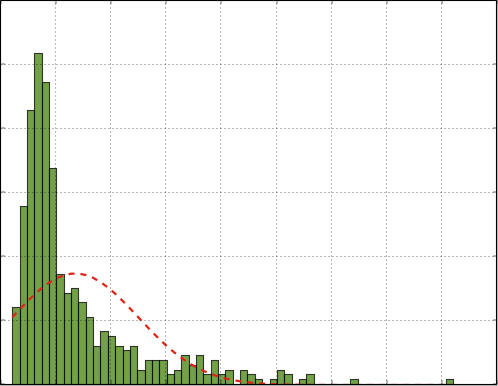
\includegraphics[width=200px]{imgs/distribucion.png}
\end{figure}


De esta forma, hemos realizado las mediciones de tiempos sobre nuestras implementaciones utilizando imágenes de distintos tamaños. Realizamos 2 analisis diferentes, uno utilizando imagenes con un mismo ancho o un mismo alto pero incrementando la otra componente, y comparando estos valores para una misma implementacion, con el fin de observar si se generaban resultados diferentes para una misma cantidad de pixeles pero con diferente organizacion. 

Para el segundo analisis y con el cual realizamos la comparación entre diferentes implementaciones utilizamos imagenes de tamaño creciente para poder observar si para diferentes cantidades de pixels los filtros mantenian la misma relacion de velocidad.
Las dimensiones utilizadas para el primer analisis fueron imagenes de 16x16*2$^{i}$ y 16*2$^{i}$x16 y para el segundo de 16*2$^{i}$x16*2$^{i}$ (con 0 $\leq$ i $\leq$ 9)

\newpage
\subsection{Cropflip}
\subsubsection{Hipótesis}
Para este filtro en particular no teniamos una idea predefinida de con que resultados nos ibamos a encontrar al realizar la experimentacion.
Al ser este un filtro muy sencillo sin necesidad de realizar operaciones matematicas en las cuales poder operar con muchos pixeles en simultaneo, la hipotesis era que la diferencia iba a estar dada por la forma de acceder a memoria pero sin esperar significativas diferencias entre una version y otra.

Elegimos tambien agregar 2 versiones extra de asm: una para medir el acceso mas simple pixel a pixel, y otra utilizando operaciones de repeticions para copiar strings, que para este caso tenia sentido aprovechar.

\subsubsection{Resultados obtenidos}

De estos resultados pudimos sacar algunas concluciones, por un lado la version de C funciono marginamlente mejor que la version asm byte a byte, por lo cual suponemos que, por lo menos en funciones en la cuales la cantidad de instrucciones dentro del ciclo es minima, no hay mucho lugar a optimizaciones posibles y el resultado es un poco mejor debido a algun mejor manejo de las variables utilizadas para iterar.

Por otro lado la version que mejor funciono fue la que utiliza la instruccion rep del microprocesador, obteniendo una ganancia del 34\% respecto a la version optimizada de C.
Incluso funciono mejor que la version simd que procesa de a 16 bytes juntos, pero que requiere mas cantidad de instrucciones para realizarlo.

De todas formas la version que utiliza simd funciono 12\% mas rapida que la version  de C con o3.


\begin{table}[!htbp]
	\centering
	\footnotesize
	\begin{tabular}{| c | c | c | c | c |}
		\hline
Pixels &asm (rep movsb)& asm (simd) & c (o3) & asm (byte a byte)\\ \hline
16x16 & 519 & 492 & 608& 821 \\ \hline
32x32  &1319  & 1594 & 2385& 2859\\ \hline
64x64  & 4430 & 5811 & 9398& 10880 \\ \hline
128x128 & 17508 & 22199 & 40104& 42483 \\ \hline
256x256  & 74415  & 100670 & 158598& 173322\\ \hline
512x512   & 272945 & 406759 & 630169& 685997 \\ \hline
1024x1024 & 2374453 & 2142237 & 4106284& 3088009 \\ \hline
2048x2048  & 10541158  & 14051375 & 15710302& 15923283\\ \hline
4096x4096 & 42235970 & 56320833 & 64179899& 65792957 \\ \hline
8192x8192 & 168890652 & 228391061 & 259152207& 266746729 \\ \hline
Tiempo en X& 1x & 1.35x & 1.53x & 1.57x  \\ \hline
Ganancia vs C & 34.83\% & 11.87\%	& 100.00\% & -2.93\% \\ \hline

 
	\end{tabular}
\end{table}


Es interesante ver que en la version con rep, como evoluciona la cantidad de clocks utilizados para procesar una imagen con la misma cantidad de pixels, pero difere si crece en ancho de si crece en alto.
Debido a que la funcion rep solo se aplica para copiar filas, se ve en la imagen como esta optimizacion mejora su relacion a medida que crece el ancho.

\begin{figure}[!h]
	\centering
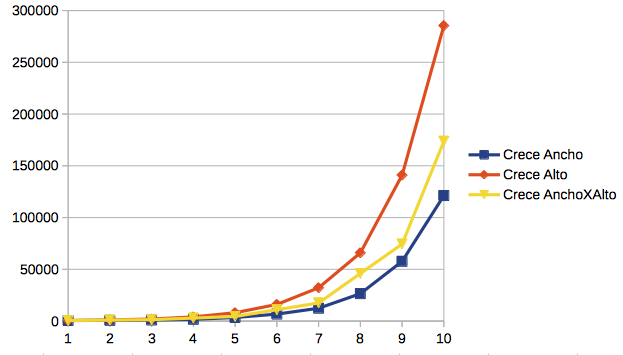
\includegraphics[width=250px]{imgs/crecimientocrop.png}
\end{figure}





\newpage
\subsection{Sepia}
\subsubsection{Hipótesis}

Para este filtro esperamos observar, como primer analisis, que las implementaciones tengan un crecimiento estable a medida que van creciendo una misma cantidad de píxeles pero con diferente organización.

Como segundo analisis, creemos que las implementaciones realizadas en ASM sean mas eficientes que la realizada en C, sin importar el tamaño de la entrada, ya que la implementación en C procesa los pixeles de manera independiente y ambas implementaciones en ASM utilizan operaciones del formato \textbf{SSE} y procesan más píxeles al mismo tiempo.

Entre las dos implementaciones de ASM, esperamos que la implementación ASM 2 (\textbf{sepia_asm2.asm}) sea levemente más eficiente frente a la implementación ASM 1 (\textbf{sepia_asm.asm}) ya que posee una operación menos para realizar los calculos sobre los pixeles y no posee una operación de división (\textbf{divps}), que si posee ASM 1.

\subsubsection{Resultados Obtenidos - Primer Analisis}

Los siguientes graficos presentan los resultados obtenidos de nuestro primer analisis en donde realizamos la comparación de cada una de las implementaciones consigo misma con el fin de observar si se generan resultados diferentes para una misma cantidad de píxeles pero con diferente organización.

\begin{figure}[h!]
	\centering
		\begin{tabular}{cc}
		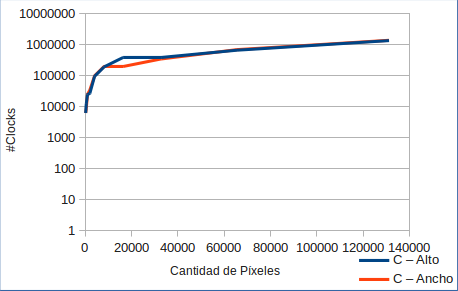
\includegraphics[width=250px]{imgs/sepia-c-analisis1.png} &
		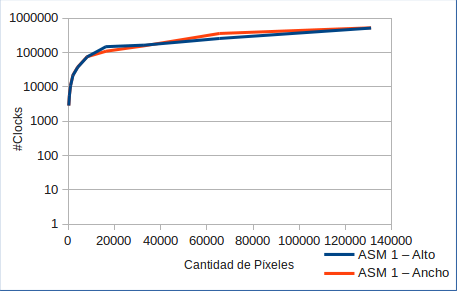
\includegraphics[width=250px]{imgs/sepia-asm1-analisis1.png} \\
		\end{tabular}
		\begin{tabular}{c}
		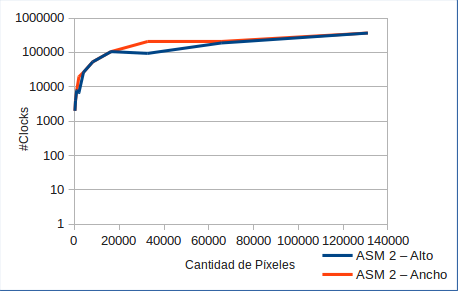
\includegraphics[width=250px]{imgs/sepia-asm2-analisis1.png} \\
		\end{tabular}
\end{figure}

Podemos observar que las curvas de crecimiento de nuestras tres implementaciones del filtro tienden a tener un mismo comportamiento a media que la cantidad de pixeles va en aumento, lo que afirma nuestra hipótesis sobre este primer analisis. Por otro lado, también puede observarse que para tamaños de entrada de entre 20000 y 40000 píxeles las tres implementaciones generar una diferencia, en alguno mas sutil como en ASM 1 y en otro mas marcada como en la de ASM 2. Este comportamiento inesperado sería interesante estudiarlo posteriormente.

\subsubsection{Resultados Obtenidos - Segundo Analisis}

Los siguientes graficos presentan los resultados obtenidos de nuestro segundo analisis en donde realizamos la comparación de performance de cada una de las implementaciones con las demás.

\begin{figure}[h!]
	\centering
	\begin{tabular}{ll}
		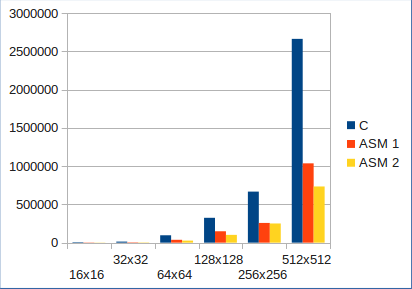
\includegraphics[width=250px]{imgs/sepia-analisis2-1.png} & 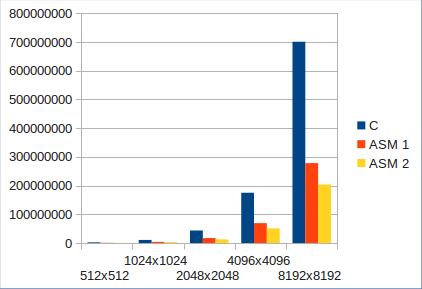
\includegraphics[width=250px]{imgs/sepia-analisis2-2.png} \\
		\vspace{1em}
	\end{tabular}
\end{figure}

Como podemos observar, la implementación en C (con O3) resultó ser mucho menos eficiente que sus contrapartes de ASM (que obtubieron ganancias del 70\% y 80\% con respecto a la implementación en C), a medida que la imagen va creciendo, esto afirma nuestra primera parte de la hipotesis. Por otro lado, entre los algoritmos ASM 1 y ASM 2 pudimos observar que se obtuvo una mas pequeña mejora en performance del ASM 2 sobre ASM 1. Esto afirma nuestra segunda parte de la hipotesis, las operaciones de división y sumas que posée la implementación ASM 1 son mucho mas costosas que las multiplicaciones que posée la implementación ASM 2 y esto se refleja en la diferencia de 0.36x superior en el tiempo de ejecución de ASM 1 con su contraparte ASM 2.

\begin{table}[!htbp]
	\centering
	\footnotesize
	\begin{tabular}{| c | c | c | c |}
		\hline
Pixels &ASM 2 & ASM 1 & C (O3) \\ \hline
16x16 & 1996 & 2862 & 6278 \\ \hline
32x32  &4232  & 4869 & 13580 \\ \hline
64x64  & 26383 & 37273 & 96682 \\ \hline
128x128 & 101613 & 148681 & 324678 \\ \hline
256x256  & 250612  & 257940 & 667089 \\ \hline
512x512   & 733971 & 1036902 & 2664477 \\ \hline
1024x1024 & 3161181 & 4314780 & 10863381 \\ \hline
2048x2048  & 12802011 & 17375403 & 43898460 \\ \hline
4096x4096 & 51152475 & 69574692 & 175335426 \\ \hline
8192x8192 & 204137541 & 278365320 & 700733874 \\ \hline
Tiempo en X& 1x & 1.36x & 3.43x \\ \hline
Ganancia vs C & 70.86\% & 60.29\%	& 100.00\% \\ \hline

	\end{tabular}
\end{table}

\newpage
\subsection{Low-Dyn Range}
\subsubsection{Hipótesis}

Para este filtro en particular, dada su complejidad, en cuanto al orden necesario para acceder en memoria a los valores, y los calculos para arrivar al resultado, hipotetizamos que la diferencia obtenida entre la mejor version de ASM y la mejor version de C serian mayores que las mismas comparaciones entre otros filtros, debido a que las optimizaciones que el compilador pudiese efectuar sobre el codigo y los accesos a memoria, no serian tan buenas como hacer un analisis especifico del funcionamiento del filtro y deduciendo que valores se puede reutilizar y que calculos se pueden realizar en paralelo utilizando instrucciones SSE.

Por otro lado realizamos 2 versiones diferentes tanto en C como en ASM con la idea de poder comparar por un lado la ganancia posible a travez de instrucciones SSE y por otro la gananica de reordenar la forma de acceso a los datos.


\subsubsection{Resultados obtenidos}


Los resultados que obtuvimos estuvieron razonablemente dentro de lo esperado. La ganancia entre la mejor version de ASM y la mejor de C con optimizacion en O3, permitiria aplicar el filtro en un poco mas de 4 imagens al mismo tiempo que la de C se lo aplica a 1 sola, o tambien, pudiendo aplicar el filtro a una imagen del doble de ancho y doble de alto (lo cual es muy util en el contexto de pantallas cada vez con mas resolucion). 

Tambien de alguna manera esperado fue que la ganancia utilizando SIMD fuese de ~4x dado que es justamente la cantidad de pixels que se pueden manejar simultaneamnte .

\begin{table}[!htbp]
	\centering
	\footnotesize
	\begin{tabular}{| c | c | c | c | c | c |}
		\hline
Pixels & ASM & C (o3) & C preproc (o3) & ASM simd & ASM simd preproc \\ \hline
16x16  & 33357 & 18596 & 13153 & 5194 & 3449 \\ \hline
32x32  & 181961 & 101292 & 62862 & 27944 & 15221 \\ \hline
64x64  & 837330 & 465902 & 289280 & 134856 & 65339 \\ \hline
128x128  & 3574572 & 1995407 & 1231802 & 548901 & 272744 \\ \hline
256x256  & 14911141 & 8238530 & 5276382 & 2274634 & 1159197 \\ \hline
512x512  & 61337662 & 34614421 & 22898444 & 9514187 & 4865965 \\ \hline
1024x1024  & 246805935 & 135432773 & 85989437 & 38506702 & 20900364 \\ \hline
2048x2048  & 996559614 & 547159461 & 348591233 & 156452341 & 90032611 \\ \hline
4096x4096  & 4139577580 & 2273534155 & 1566227645 & 639810532 & 363950690 \\ \hline
8192x8192  & 16999317092 & 9493848236 & 6354314134 & 2644797660 & 1533749148 \\ \hline
Relacion & 11.0835054834 & 6.1899615386 & 4.1429944018 & 1.7244004102 & 1 \\ \hline

	\end{tabular}
\end{table}


\begin{figure}[!h]
	\centering
	\begin{minipage}{.5\textwidth}
		\centering
		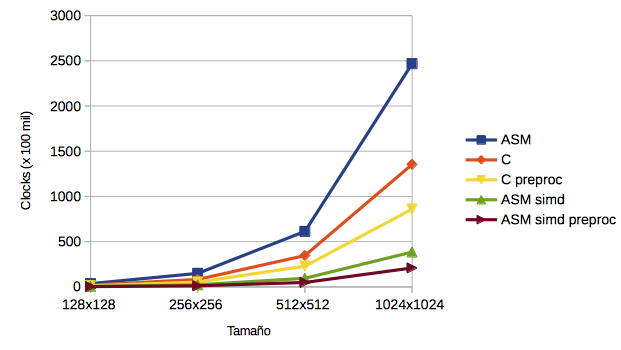
\includegraphics[width=\linewidth]{imgs/ldrTotales1.png}
	\end{minipage}\hfill
	\begin{minipage}{.5\textwidth}
		\centering
		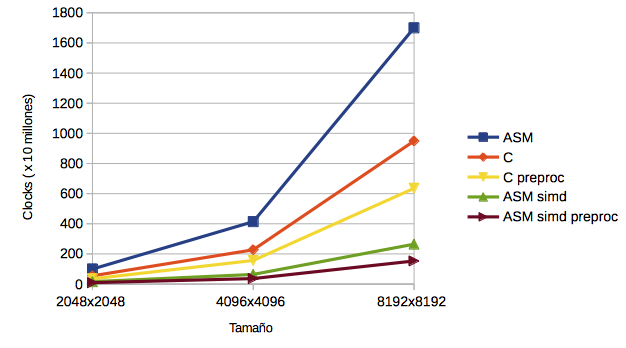
\includegraphics[width=\linewidth]{imgs/ldrTotales2.png}
	\end{minipage}\hfill
\end{figure}
 

\newpage

A su vez pudimos observar el poder de la optimizacion de C, ya que sin ningun esfuerzo de parte del programdor se obtiene una ganacia muy interesante, sobrepazando inclusive la version realizada en asm que no utilizaba instrucciones de SIMD.


\begin{figure}[!h]
	\centering
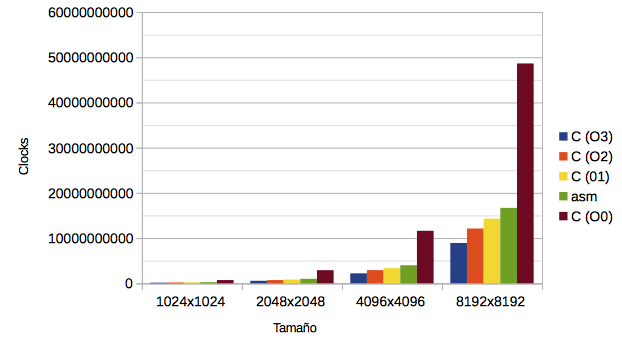
\includegraphics[width=300px]{imgs/ldrOptC.png}
\end{figure}




Dentro de los experimentos que decidimos realizar, nos preguntamos si existiria alguna diferencia en el el tiempo utilizado por los algoritmos dependiendo del parametro alpha, dado que se utiliza para multiplicar cada pixel.
Es interesante ver como se ve en el resultado de esta imagen, que para el valor de alpha=0, la cantidad de clocks utilizado, por los algoritmos que utilizan floats para la multiplicacion, diminuye significativamente. 
De esto se pueden sacar varias conclusiones interesantes, por un lado que la multiplicacion por el alpha consume una parte muy importante del tiempo total utilizado por el algoritmo.
Que si el valor es 0, el procesador resuelve inmediatamente el resultado y ademas que para el resto de los valores, no hay diferencia segun el valor por el cual se multiplique.

\begin{figure}[!h]
	\centering
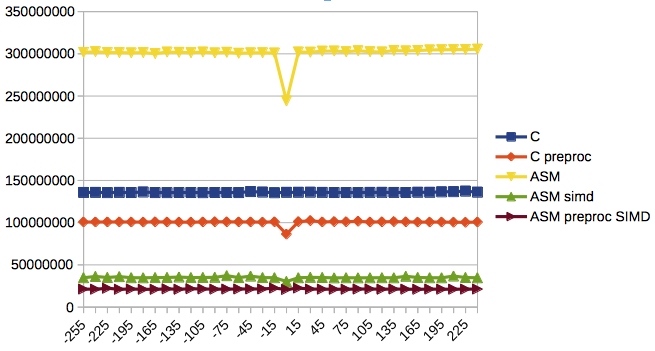
\includegraphics[width=300px]{imgs/comparacionLDR.png}
\end{figure}


\newpage

%\begin{figure}
%  \begin{center}
%	\includegraphics[scale=0.66]{imagenes/logouba.jpg}
%	\caption{Descripcion de la figura}
%	\label{nombreparareferenciar}
%  \end{center}
%\end{figure}


%\paragraph{\textbf{Titulo del parrafo} } Bla bla bla bla.
%Esto se muestra en la figura~\ref{nombreparareferenciar}.



%\begin{codesnippet}
%\begin{verbatim}

%struct Pepe {

%    ...

%};

%\end{verbatim}
%\end{codesnippet}


\section{Conclusión} 
Gracias a los experimentos de este trabajo, pudimos observar las ventajas de el modelo de procesamiento SIMD a la hora de implementar programas que realicen operaciones paralelizables, tanto en comparación con las implementaciones en C como entre las del lenguaje de ensamblador.

Por un lado, se puede observar que la performance que tienen las implementaciones en lenguaje de ensamblador con el modelo de procesamiento SIMD fue muy superior en estos casos a las implementaciones en C, que sólo procesan píxeles de forma independiente, incluso estando optimizadas con O3. 

Por otro lado, también pudimos observar que realizando las mismas funciones en lenguage de ensamblador con el modelo de procesamiento SIMD pero con algunas modificaciones en las operaciones de los mismas generan mejoras de performance, aunque no tan notorias en este caso en comparación con las implementaciones de C. 

Esto nos llevo a repensar como generar mejoras de performance en nuestras implementaciones. 
Quedaria pendiente para otro analisis, un trabajo mas detallado de comparacion entre distintas formas de utilizar simd, para encontrar metodos mas eficientes para resolver problemas comunes, como el desempaquetado de datos, operaciones aritmeticas, utilizacion de punto flotantes o enteros, etc y la identificaciones de instrucciones particularmente costosas y formas de mitigar su impacto.

Por último, quda claro que realizar un programa en lenguaje de ensamblador es mas costoso en tiempo humano, que realizarlo en un lenguaje de más alto nivel. Por este motivo es evidente que la utilizacion de ASM y SIMD en particular, quedan restringidas a situaciones donde la ganancia de utilizar este metodo justifique el esfuerzo invertido.



\end{document}

